\chapter{An Example \simplesine Simulation}
\label{sec:simplesine-sim}

In the following chapters,
we use the \simplesine model extensively as part of simulations
to illustrate \TrickHLA\ in action.
In this chapter, we introduce a non-HLA \simplesine simulation
as a way to explain the basics of how the model may be used with Trick,
and we do so without any \TrickHLA\ distractions.

% ----------
\section{\tt SIM\_simplesine\_pubsub}

In this simulation, there are two {\tt sim\_object}s:
a {\em publisher} and a {\em subscriber}.\footnote{
This publisher/subscriber terminology here is only suggestive.
There is no distributed computing going on.
Data only moves from one {\tt sim\_object} to another within a single process.
Nevertheless, the simulation is a fair way to introduce how \simplesine
data structure and functions are used in Trick \sdefine and input files.
}
The publisher generates a sine wave using the analytic equations
and periodically copies the state to the subscriber.
The subscriber propagates the state approximately between updates from
the publisher.
Based on the analytic equations, the subscriber also calculates an error
in the approximate propagation.

The motivation for having the publisher and subscriber propagate the state
differently is to illustrate a technique that is useful for HLA simulations.
The owner of some data might simulate it at a very high rate but
send updates at a lower frequency.
In between these updates, a subscriber may use an approximate method to
extrapolate the data until the next update arrives.\footnote{
  Extrapolation alternatives include doing nothing, in which case the
  data increments in discontinuous steps as the remote data arrive;
  dead reckoning, in which the data are extrapolated based on derivatives;
  or numerical integration of an approximate (lower fidelity) model, in
  which case the discontinuities on the subscriber side are hopefully
  reduced sufficiently to allow the subscriber's simulation to proceed.
}
% ----------
\section{\sdefine}
\label{sec:simplesine-pubsub-sdefine}

The {\tt SIM\_simplesine\_pubsub} \sdefine file is shown below. It consists of

\begin{itemize}
  \item{
    Some {\tt \#define} statements that set relevant frequencies for
    state propagation and data copying.
  }
  \item{
    The {\tt sim\_object}s -- the usual Trick {\tt sys} object and
    publisher and subscriber objects.
  }
  \item{
    An {\tt integrate} statement which enables Trick numerical integration
    for the subscriber.
  }
\end{itemize}

\begin{lstlisting}[caption={{\tt SIM\_simplesine\_pubsub} \sdefine file},label={list:SIM-pubsub-sdefine}]
#define PROPAGATE_TIMESTEP 0.25
#define COPY_TIMESTEP 5.0

sim_object
{
  sim_services/include: EXECUTIVE exec (sim_services/include/executive.d) ;

  (automatic) sim_services/input_processor:
    input_processor( INPUT_PROCESSOR* IP = &sys.exec.ip ) ;
} sys ;


sim_object
{
  simplesine: simplesine_T simplesine (simplesine/data/simplesine.d);

  (initialization) simplesine:
    simplesine_calc(
      simplesine_T* P = &publisher.simplesine,
      double t = sys.exec.out.time );

  // Propagate the state using the analytic equations.
  (PROPAGATE_TIMESTEP, scheduled) simplesine:
    simplesine_calc(
      simplesine_T* P = &publisher.simplesine,
      double t = sys.exec.out.time );

  // Copy the propagated state to the subscriber.
  (COPY_TIMESTEP, scheduled) simplesine:
    simplesine_copyState(
      simplesine_state_T* fromP = &publisher.simplesine.state,
      simplesine_state_T* toP = &subscriber.simplesine.state );
} publisher ;


sim_object
{
  sim_services/include: INTEGRATOR integ (simplesine/data/integ.d);
  simplesine: simplesine_T simplesine (simplesine/data/simplesine.d);
  simplesine: simplesine_T err (simplesine/data/simplesine.d);

  (initialization) simplesine:
    simplesine_calc(
      simplesine_T* P = &subscriber.simplesine,
      double t = sys.exec.out.time );

  // deriv/integ jobs to propagate the state differential equation
  (derivative) simplesine:
    simplesine_deriv( simplesine_T* p = &subscriber.simplesine );
  (integration) simplesine:
    simplesine_integ(
      INTEGRATOR* I = &subscriber.integ,
      simplesine_T* p = &subscriber.simplesine );

  // calculate the error between the integrated state and the true state
  (PROPAGATE_TIMESTEP, scheduled) simplesine:
    simplesine_calcError(
      double t = sys.exec.out.time,
      simplesine_T* s = &subscriber.simplesine,
      simplesine_state_T* err = &subscriber.err.state );
} subscriber ;

integrate (PROPAGATE_TIMESTEP) subscriber;
\end{lstlisting}
% ----------
\section{Input Files}

The input files for this simulation are located in the {\tt RUN\_1} directory
and are summarized below.

\begin{itemize}
\item{
  {\tt input\_noCopy\_noInteg}.
  In this input file,
  the publisher never sends data to the subscriber, and
  the subscriber does not propagate its local state.
  The motivation here is to illustrate that nothing really happens
  on the subscriber side until the publisher sends data.
}
\item{
  {\tt input\_noInteg}.
  This input file illustrates the arrival of data at the subscriber from
  the publisher.
  By not propagating the subscriber state, the discrete arrival of
  updates is readily evident.
  In some simulations in the subsequent chapter,
  we will use this technique to illustrate the arrival of HLA data.
}
\item{
  {\tt input}.
  This file illustrates the simulation running as it is intended:
  the publisher sends data periodically to the subscriber,
  and the subscriber integrates those data in between updates.
  In this case the harmonical oscillator is so simple that the numerical
  integration is a very good approximation to the true system.
}
\end{itemize}

The first two files illustrate how to disable specific Trick jobs from
the input file using the {\tt JOB} directive.
In {\tt input\_noCopy\_noInteg}, the publisher's
publisher-to-subscriber copy job is disabled
as well as the subscriber's numerical integration jobs.
In {\tt input\_noInteg}, the subscriber's numerical integration jobs are
disabled.
The input files are shown below.


\begin{lstlisting}[caption={{\tt SIM\_simplesine\_pubsub} input file, {\tt input\_noCopy\_noInteg}},label={list:SIM-pubsub-input-noCopy-noInteg}]
#include "S_default.dat"
#include "Log_data/states.d"
#include "Modified_data/realtime.d"
#include "Modified_data/publisher.d"
#include "Modified_data/subscriber.d"

JOB publisher.simplesine_copyState(&publisher.simplesine) = Off;

JOB subscriber.simplesine_deriv(&subscriber.simplesine) = Off;
JOB subscriber.simplesine_integ(&subscriber.integ) = Off;

stop = 32.5;
\end{lstlisting}

\begin{lstlisting}[caption={{\tt SIM\_simplesine\_pubsub} input file, {\tt input\_noInteg}},label={list:SIM-pubsub-input-noInteg}]
#include "S_default.dat"
#include "Log_data/states.d"
#include "Modified_data/realtime.d"
#include "Modified_data/publisher.d"
#include "Modified_data/subscriber.d"

JOB publisher.simplesine_copyState(&publisher.simplesine) = Off;

stop = 32.5;
\end{lstlisting}

\begin{lstlisting}[caption={{\tt SIM\_simplesine\_pubsub} input file, {\tt input}},label={list:SIM-pubsub-input}]
#include "S_default.dat"
#include "Log_data/states.d"
#include "Modified_data/realtime.d"
#include "Modified_data/publisher.d"
#include "Modified_data/subscriber.d"

stop = 32.5;
\end{lstlisting}

% ----------
\section{Output}

Output from the simulation with {\tt input\_noCopy\_noInteg}
is shown in Figure~\ref{fig:SIM-pubsub-input-noCopy-noInteg}.
The plot shows the evolution of the sine wave for approximately
ten cycles.
The publisher state ($x(t)$ and $\dot{x}(t)$) evolve as expected.
The subscriber state is flatlined at its initial conditions,
since data never arrive from the publisher and the subscriber's
numerical propagation is disabled.

\begin{figure}[b]
  \begin{center}
    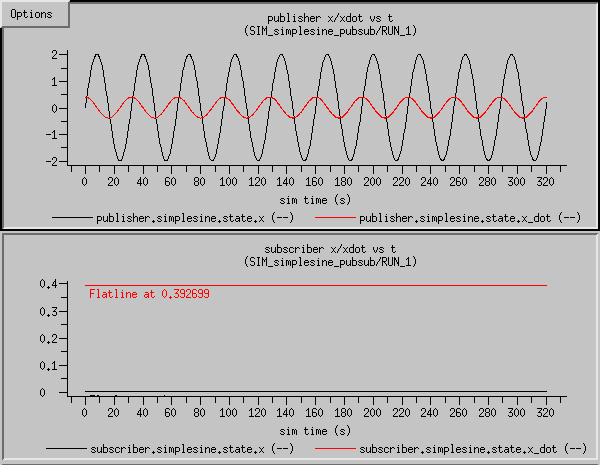
\includegraphics[width=4.5in]{TrickHLAUser-prelim-SIM-pubsub-input-noCopy-noInteg.png}
  \end{center}
\caption{Output from {\tt SIM\_simplesine\_pubsub} using input file {\tt input\_noCopy\_noInteg}}
\label{fig:SIM-pubsub-input-noCopy-noInteg}
\end{figure}


Output from the simulation with {\tt input\_noInteg}
is shown in Figure~\ref{fig:SIM-pubsub-input-noInteg}.
It clearly shows the discrete transfer of data from the publisher to the
subscriber.
Between the data updates, the subscriber state remains constant,
since there is still no numerical intregration on the subscriber side.
This manifests itself in errors which grow significantly until the next
update arrives, at which point the errors reset to zero.

\begin{figure}[b]
  \begin{center}
    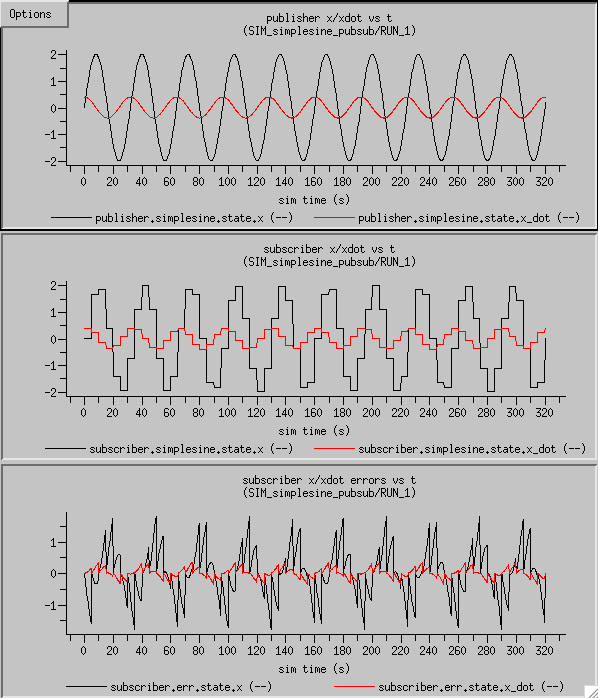
\includegraphics[width=4.5in]{TrickHLAUser-prelim-SIM-pubsub-input-noInteg.png}
  \end{center}
\caption{Output from {\tt SIM\_simplesine\_pubsub} using input file {\tt input\_noInteg}}
\label{fig:SIM-pubsub-input-noInteg}
\end{figure}


Output from the simulation with {\tt input}
is shown in Figure~\ref{fig:SIM-pubsub-input}.
In this case, the subscriber state is ``smoothed'' in between data updates,
since the subscriber numerical integration has been enabled.
Note that there are still errors which grow between updates;
however, in this case the magnitude of those error has diminished by several
orders of magnitude.

\begin{figure}[b]
  \begin{center}
    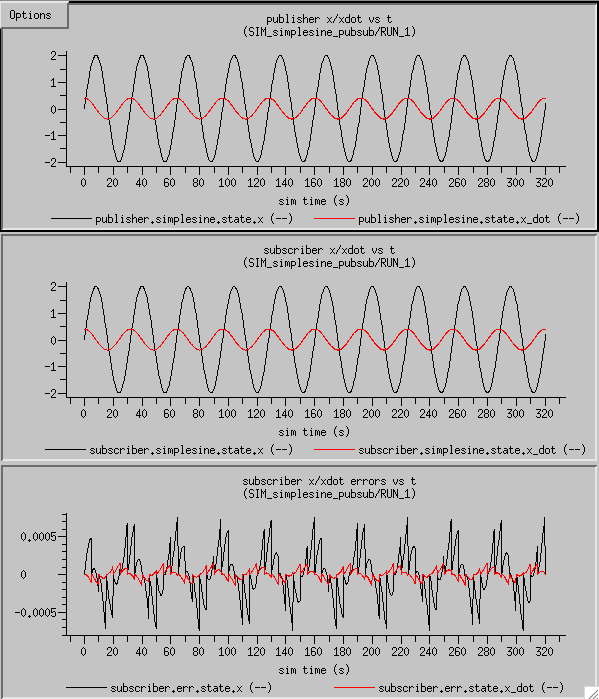
\includegraphics[width=4.5in]{TrickHLAUser-prelim-SIM-pubsub-input.png}
  \end{center}
\caption{Output from {\tt SIM\_simplesine\_pubsub} using input file {\tt input}}
\label{fig:SIM-pubsub-input}
\end{figure}

%
% print the figures before moving to the next chapter
%
\clearpage
